%%% LaTeX Template: Article/Thesis/etc. with colored headings and special fonts
%%%
%%% Source: http://www.howtotex.com/
%%% Feel free to distribute this template, but please keep to referal to http://www.howtotex.com/ here.
%%% February 2011
%%%
%%% Modified May 2018 by CDM

%%%  Preamble
\documentclass[11pt,letterpaper]{article}
\usepackage[margin=1.0in]{geometry}
\usepackage[T1]{fontenc}
\usepackage[bitstream-charter]{mathdesign}
\usepackage[latin1]{inputenc}					
\usepackage{amsmath}						
\usepackage{xcolor}
\usepackage{cite}
\usepackage{hyphenat}
\usepackage{graphicx}
\usepackage{float}
\usepackage{subfigure}
\usepackage{sectsty}
\usepackage[compact]{titlesec} 
\usepackage[tablegrid]{vhistory}
\allsectionsfont{\color{accentcolor}\scshape\selectfont}

%%% Definitions
\definecolor{accentcolor}{rgb}{0.0,0.0,0.5} 
\newcommand{\teamname}{Team 10}
\newcommand{\productname}{MedTech}
\newcommand{\coursename}{CSE 4316: Senior Design I}
\newcommand{\semester}{Fall 2020}
\newcommand{\docname}{System Requirements Specification}
\newcommand{\department}{Department of Computer Science \& Engineering}
\newcommand{\university}{The University of Texas at Arlington}
\newcommand{\authors}{Maxwell Pham\\Nikita Menon\\Hemantha Govindu\\Nisarg Shah}

%%% Headers and footers
\usepackage{fancyhdr}
	\pagestyle{fancy}						% Enabling the custom headers/footers
\usepackage{lastpage}	
	% Header (empty)
	\lhead{}
	\chead{}
	\rhead{}
	% Footer
	\lfoot{\footnotesize \teamname \ - \semester}
	\cfoot{}
	\rfoot{\footnotesize page \thepage\ of \pageref{LastPage}}	% "Page 1 of 2"
	\renewcommand{\headrulewidth}{0.0pt}
	\renewcommand{\footrulewidth}{0.4pt}

%%% Change the abstract environment
\usepackage[runin]{abstract}			% runin option for a run-in title
%\setlength\absleftindent{30pt}			% left margin
%\setlength\absrightindent{30pt}		% right margin
\abslabeldelim{\quad}	
\setlength{\abstitleskip}{-10pt}
\renewcommand{\abstractname}{}
\renewcommand{\abstracttextfont}{\color{accentcolor} \small \slshape}	% slanted text

%%% Start of the document
\begin{document}

%%% Cover sheet
{\centering \huge \color{accentcolor} \sc \textbf{\department \\ \university} \par}
\vspace{1 in}
{\centering \huge \color{accentcolor} \sc \textbf{\docname \\ \coursename \\ \semester} \par}
\vspace{0.5 in}
\begin{figure}[h!]
	\centering
   	
\includegraphics[width=0.40\textwidth]{images/Apollo}
\end{figure}
\vspace{0.5 in}
{\centering \huge \color{accentcolor} \sc \textbf{\teamname \\ \productname} \par}
\vspace{0.5 in}
{\centering \large \sc \textbf{\authors} \par}
\newpage


%\vspace{1 in}
%\centerline{January 13th, 2012}
%\newpage

%%% Revision History
\begin{versionhistory}
  	\vhEntry{0.1}{10.08.2020}{MP}{document creation}
  	\vhEntry{0.2}{10.17.2020}{MP}{Added Product Concept}
  	\vhEntry{0.2.1}{10.18.2020}{MP}{Added Safety Requirements}
  	\vhEntry{0.2.3}{10.23.2020}{MP}{Added Future Requirements, updated Safety Req.}
  	\vhEntry{0.3}{10.24.2020}{MP|NM|HG|NS}{release candidate 1}
  	\vhEntry{1.0}{10.28.2020}{NM}{Official Release}
\end{versionhistory}
\newpage

%%% Table of contents
\setcounter{tocdepth}{3}
\tableofcontents
\newpage

%%% List of figures and tables (optional)
\listoffigures
%\listoftables
\newpage

\section{Product Concept}
This section provides a high-level statement of your product concept - what it is intended to do and how it is intended to be used. Include in this header paragraph, a brief synopsis of what is described here. For example, this header paragraph might say something like: "This section describes the purpose, use and intended user audience for the X product. X is a system that performs Y. Users of X will be able to Z..."

\subsection{Purpose and Use}
This is where you describe in a brief, yet clear and concise, manner what your product should do and how you expect it should be used.

\subsection{Intended Audience}
This is where you describe the intended audience(s) of your product. If this product were to be made available publicly or commercially, who would purchase or use it? Is the product designed for a particular customer, or an overall class of customers? Is it intended for general use, or is it a specific component of a more complex system?

\begin{figure}[h!]
	\centering
   	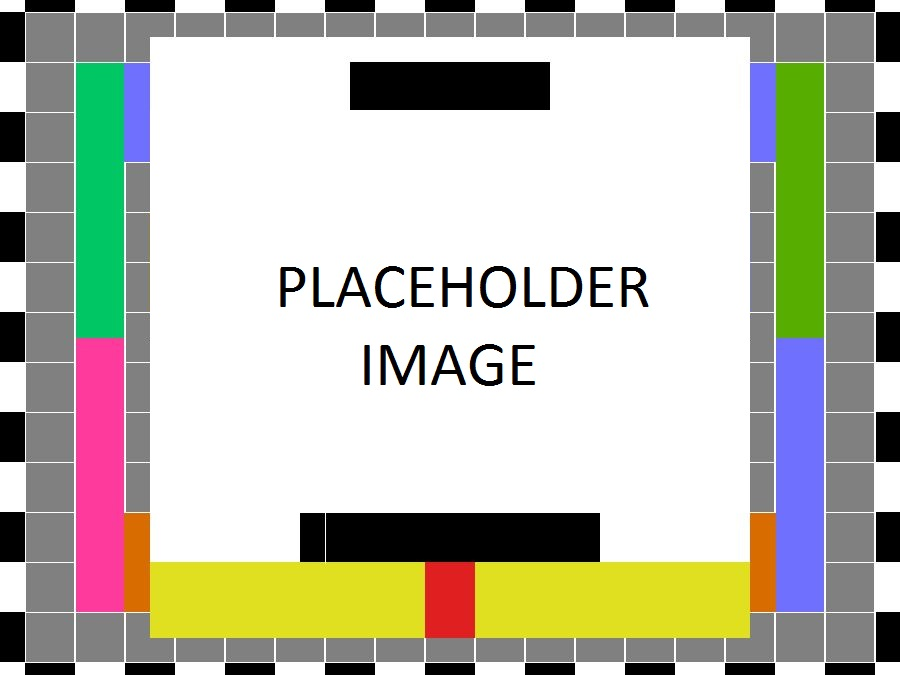
\includegraphics[width=0.60\textwidth]{images/test_image}
    \caption{X conceptual drawing}
\end{figure}

\newpage
\section{Product Description}
This section provides a brief description of features of MedTech. The primary operational aspects is it to assist medical professionals with the health care of patients. MedTech aims to increase efficiency and usability of EMR systems. This section provides the reader with an overview of our EMR System, MedTech. Below we outline the key features and functions found in the products as well as critical user interactions and user interfaces from the perspective of end users, maintainers and administrators. 

\subsection{Features \& Functions}

The main features we hope to target are: 

1) Hourly updates from patient to health care professionals 

2) Voice recognition verification from doctors to patients for medications, prescriptions 

3) Patient history details like previous ailments, medications, prescriptions, allergies and others. 

4) Integration of machine learning and other deep learning models to help with early diagnosis 

5) Updating lab results and other diagnostics in to the software 

6) Conversion of notes from medical professionals to billing and other document management. 

Since the medical field is a diverse industry and includes a variety of specializations, we will be focusing on a select department so as to narrow down our focus. 





\section{Sprint Backlog}
External inputs and outputs are outlined in the table below:  \\ % work units do not have to be hours, change text accordingly


\begin{tabular}{| p{1in} | >{\centering\arraybackslash} p{2in} | >{\centering\arraybackslash} p{2in} |}
\hline
NAME & DESCRIPTION & USE \\ \hline
Login & A login page for medical professionals & To login with their credentials  \\ \hline
Patient File Summary & Brief description of patient's file & This would display patient basic information, allergies, ID and blood type \\ \hline
Patient Updates & Updates by doctors,pharmacy and other health care professionals  & This would include updates to treatment plan,pharmacy prescriptions and other orders from doctors \\ \hline
Settings & This would be to help with UI/basic web settings & Provide users with options to change password and other basic operations \\ \hline
Logout & A button to exit  & This will logout out of professional's particular page. \\ \hline
Other elements & elements pertaining to individual patients & It would include patient for lab,flowsheet, patient history and updates all would appear on the same page \\ \hline

\end{tabular}
\pagebreak

\subsection{Product Interfaces}
Below we have mock ups for our login page and patient file summary. 

\begin{figure}[h!]
	\centering
   	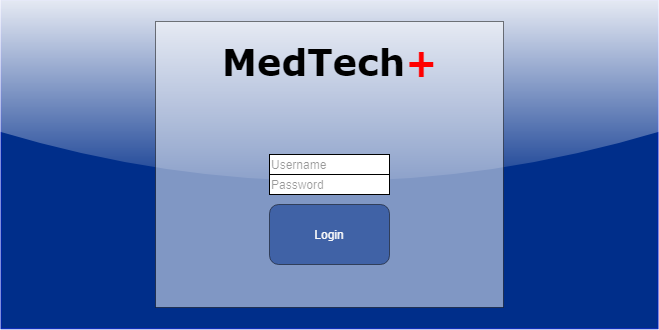
\includegraphics[width=1.00\textwidth]{images/Login.png}
    \caption{Login}
\end{figure}

\begin{figure}[h!]
	\centering
   	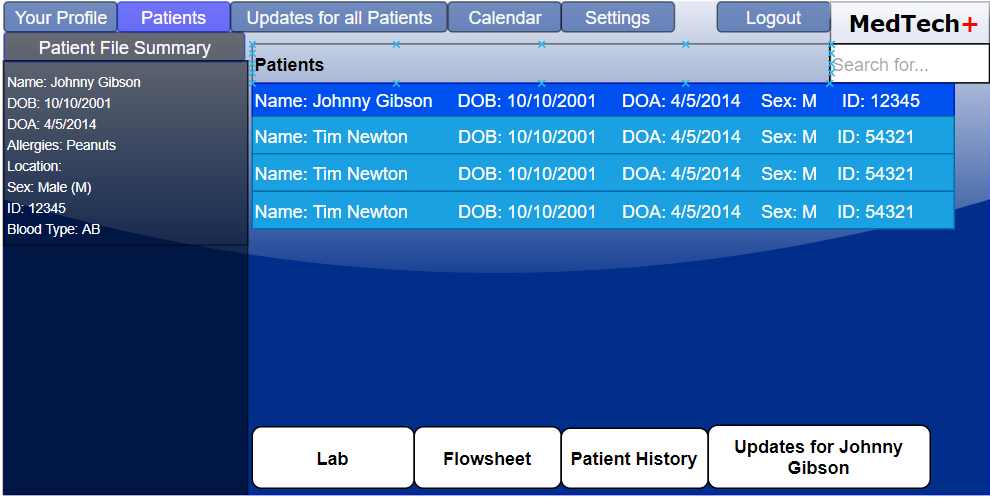
\includegraphics[width=1.00\textwidth]{images/afterlogin.PNG}
    \caption{After Login}
\end{figure}
\newpage
\section{Customer Requirements}

This project is meant to serve the medical community with helping them minimize the charting time. So this project will mainly be focused on improving the UI/UX and smarter layout for application with collective effort to make a seamless integration of state-of-the art technologies meant to help maximize the readability of the system as compared to the industry standard of software such as Epic. 

\subsection{Log-in for medical staff}
\subsubsection{Description}
The medical staff like nurses and doctors should be able to create their unique account and then later log-in with that. Every employee should have one and only one account.
\subsubsection{Source}
Sponsors ( Medical Professional/students )
\subsubsection{Constraints}
No sensitive information should be displayed on the screen without the staff member changing their temporary password.
\subsubsection{Standards}
NIST standard fir password management
\subsubsection{Priority}
High

\subsection{Log tracking}
\subsubsection{Description}
The system should be able to log each and every action taken to modify or view sensitive data for legal purposes and to satisfy one of the HIPPA rules
\subsubsection{Source}
Team
\subsubsection{Constraints}
Constraints include verifying the log status without increasing too much latency
\subsubsection{Standards}
HIPPA
\subsubsection{Priority}
High 

\subsection{Lab reports integration}
\subsubsection{Description}
The system should allow integration of lab reports of medical patient for the nurses and doctors to view in the same patient profiles along with their other details as mentioned in the below requirement
\subsubsection{Source}
Team, sponsor
\subsubsection{Constraints}
The lab report integration should be in real time but that blocks off some computation power and might increase cost.
\subsubsection{Standards}
HIPPA
\subsubsection{Priority}
High 


\subsection{Patient History }
\subsubsection{Description}
The system should be able to store and collect patient data from medical professional to help them with their analysis.
\subsubsection{Source}
Team
\subsubsection{Constraints}
More data to handle in out database, can increase the search-time
\subsubsection{Standards}
HIPPA
\subsubsection{Priority}
High 

\subsection{Charting}
\subsubsection{Description}
The system should be able to provide an interface to staff members to chart their health including but not limited to daily vitals.
\subsubsection{Source}
Sponsors ( Medical Professional/students )

\subsubsection{Constraints}
Need to keep many check statements, a bug might prevent them from charting properly.
\subsubsection{Standards}
HIPPA
\subsubsection{Priority}
High 

\newpage
\section{Packaging Requirements}
Include a header paragraph here. Packaging requirements are those requirements that identify how the delivered product will be packaged for delivery to the end-user; or how it will "look" when finished and delivered. For example, you might specify that the software required for operation will be pre-loaded on the hard drive, delivered on CD/DVD, or available via download. Software might be customer installable, or not, etc. Hardware components could be all in a single package, provided as a "bag of parts" to be assembled/installed by the user, painted a certain color, logos affixed, etc. Care should be taken not to duplicate requirements found in other sections of this document.

\subsection{Requirement Name}
\subsubsection{Description}
Detailed requirement description...
\subsubsection{Source}
Source
\subsubsection{Constraints}
Detailed description of applicable constraints...
\subsubsection{Standards}
List of applicable standards
\subsubsection{Priority}
Priority
\newpage
\section{Performance Requirements}
The main goal of this project will be to minimize the amount to time medical professionals spend charting and remove some of the unnecessary steps in between. 

\subsection{Always on service}
\subsubsection{Description}
Since this project will be dealing with EMR( Electronic Medical Record ) and EHR ( electronic Health Record ) system, this service should be available 24 hours a day and 365 days a year.
\subsubsection{Source}
Team
\subsubsection{Constraints}
Constraints include: 
1) Assuming AWS or any other service provide are providing service with 100 percent performance time
\subsubsection{Standards}
None
\subsubsection{Priority}
Low

\subsection{Reliability}
\subsubsection{Description}
The client side service should never break or exit without explicit action taken by the user/customer
\subsubsection{Source}
Team
\subsubsection{Constraints}
Constraints may include hardware issues
\subsubsection{Standards}
None
\subsubsection{Priority}
High
\newpage
\section{Safety Requirements}
Medtech is mainly a software project that will not require the use of laboratory equipment.

\subsection{Laboratory equipment lockout/tagout (LOTO) procedures}
\subsubsection{Description}
Any fabrication equipment provided used in the development of the project shall be used in accordance with OSHA standard LOTO procedures. Locks and tags are installed on all equipment items that present use hazards, and ONLY the course instructor or designated teaching assistants may remove a lock. All locks will be immediately replaced once the equipment is no longer in use.
\subsubsection{Source}
CSE Senior Design laboratory policy
\subsubsection{Constraints}
Equipment usage, due to lock removal policies, will be limited to availability of the course instructor and designed teaching assistants.
\subsubsection{Standards}
Occupational Safety and Health Standards 1910.147 - The control of hazardous energy (lockout/tagout).
\subsubsection{Priority}
Non-existent

\subsection{No inaccuracies of charted data}
\subsubsection{Description}
For legal reasons and patient safety, charted data must be absolutely accurate and must be double checked. Charted data includes medication orders for the correct drug and its prescription.
\subsubsection{Source}
The Office of the National Coordinator for Health Information Technology, Reducing Medication Errors: Simple Recommendations
\subsubsection{Constraints}
Software usage may be limited without training or reference to a nurse's inputs.
\subsubsection{Standards}
Tools: Reducing Pick List Errors in Medication Ordering for Providers \cite{AndrewGettinger2016}
\subsubsection{Priority}
High


\newpage
\section{Maintenance \& Support Requirements}
Include a header paragraph specific to your product here. Maintenance and support requirements address items specific to the ongoing maintenance and support of your product after delivery. Think of these requirements as if you were the ones who would be responsible for caring for customers/end user after the product is delivered in its final form and in use "in the field". What would you require to do this job? Specify items such as: where, how and who must be able to maintain the product to correct errors, hardware failures, etc.; required support/troubleshooting manuals/guides; availability/documentation of source code; related technical documentation that must be available for maintainers; specific/unique tools required for maintenance; specific software/environment required for maintenance; etc.

\subsection{Requirement Name}
\subsubsection{Description}
Detailed requirement description...
\subsubsection{Source}
Source
\subsubsection{Constraints}
Detailed description of applicable constraints...
\subsubsection{Standards}
List of applicable standards
\subsubsection{Priority}
Priority
\newpage
\section{Other Requirements}
Include a header paragraph specific to your product here. In this section specify anything else that is required for the product to be deemed complete. Include requirements related to customer setup and configuration if not specified in a previous requirement. Add any known requirements related to product architecture/design, such as modularity, extensibility (for future enhancements), or adaptation for a specific programming language. Consider requirements such as portability of your source code to various platforms (Windows, Linux, Unix Mac OS, etc.).

\subsection{Requirement Name}
\subsubsection{Description}
Detailed requirement description...
\subsubsection{Source}
Source
\subsubsection{Constraints}
Detailed description of applicable constraints...
\subsubsection{Standards}
List of applicable standards
\subsubsection{Priority}
Priority
\newpage
\section{Future Items}
\subsection{Health Information Technology for Economic and Clinical Health (HITECH) Act of 2009}
\subsubsection{Description}
Provides the HHS (US Dpt. of Health \& Human Services) authority to establish programs to improve health care quality, safety, and efficiency through the promotion of health IT. This includes electronic health records and privately secured electronic health information exchange.
\subsubsection{Source}
Index for Excerpts from the American Recovery and Reinvestment Act of 2009 (ARRA)
\subsubsection{Constraints}
MedTech EHR must employ "(2) ENTERPRISE INTEGRATION" meaning the electronic linkage of health care providers, health plans, the government, and other interested parties, to enable the electronic exchange and use of health information among all components of the health care infrastructure.
\subsubsection{Standards}
SEC. 13101. ONCHIT; STANDARDS DEVELOPMENT AND ADOPTION. \cite{UnitedStatesCongress2009}
\subsubsection{Priority}
Moderate

\subsection{Health Insurance Portability and Accountability Act (HIPAA) of 1996}
\subsubsection{Description}
This protects health insurance coverage for workers and their families when they change or lose their jobs, requires the establishment of national standards for electronic health care transactions, and requires establishment of national identifiers for providers, health insurance plans, and employers.
\subsubsection{Source}
HEALTH INSURANCE PORTABILITY AND ACCOUNTABILITY ACT OF 1996 Public Law 104-191 104th Congress
\subsubsection{Constraints}
Patients must have insurance entries and will be viewed for money billing and transactions.
\subsubsection{Standards}
TITLE XXVII--ASSURING PORTABILITY, AVAILABILITY, AND RENEWABILITY OF HEALTH INSURANCE COVERAGE \cite{Caplan2003}
\subsubsection{Priority}
Low
\newpage

%%% References
\bibliographystyle{plain}
\bibliographystyle{reference/IEEEtran_custom}
\bibliography{reference/refs}{}

\end{document}